\subsection{HDR ML Anomaly Challenge - Butterfly}
{{\footnotesize
\noindent Image-based challenge for detecting butterfly hybrids in microscopy-driven species data. Participants evaluate models on Codabench using image segmentation/classification. 


\begin{description}[labelwidth=4cm, labelsep=1em, leftmargin=4cm, itemsep=0.1em, parsep=0em]
  \item[date:] 2025-03-03
  \item[version:] v1.0
  \item[last\_updated:] 2025-03
  \item[expired:] unknown
  \item[valid:] yes
  \item[valid\_date:] 2025-03-03
  \item[url:] \href{https://www.codabench.org/competitions/3764/}{https://www.codabench.org/competitions/3764/}
  \item[doi:] 10.48550/arXiv.2503.02112
  \item[domain:]
    - Biology \& Medicine
  \item[focus:] Detecting hybrid butterflies via image anomaly detection in genomic-informed dataset
  \item[keywords:]
    - anomaly detection
    - computer vision
    - genomics
    - butterfly hybrids
  \item[licensing:] NA
  \item[task\_types:]
    - Anomaly Detection
  \item[ai\_capability\_measured:]
    - Hybrid detection in biological systems
  \item[metrics:]
    - Classification accuracy
    - F1 score
  \item[models:]
    - CNN-based detectors
  \item[ml\_motif:]
    - Anomaly Detection
  \item[type:] Dataset
  \item[ml\_task:]
    - Anomaly Detection
  \item[solutions:] Solution details are described in the referenced paper or repository.
  \item[notes:] Hybrid detection benchmarks hosted on Codabench

  \item[contact.name:] Imageomics/HDR Team
  \item[contact.email:] unknown
  \item[results.links.name:] ChatGPT LLM
  \item[fair.reproducible:] Yes
  \item[fair.benchmark\_ready:] Yes
  \item[id:] hdr\_ml\_anomaly\_challenge\_-\_butterfly
  \item[Citations:] \cite{campolongo2025buildingmachinelearningchallenges2}
\end{description}

{\bf Ratings:} ~ \\

\begin{tabular}{p{0.15\textwidth} p{0.07\textwidth} p{0.7\textwidth}}
\hline
Rating & Value & Reason \\
\hline
dataset & 3 & Dataset consists of real detector data with synthetic anomaly injections; access
is restricted and requires NDA, limiting openness and FAIR compliance.
 \\
documentation & 3 & Challenge website provides basic descriptions and evaluation metrics but lacks
comprehensive tutorials or example workflows.
 \\
metrics & 3 & Standard metrics (ROC, F1, precision) are used; evaluation protocols are clear
but not deeply elaborated.
 \\
reference\_solution & 2 & Baselines are partially described but lack public code or reproducible execution
scripts.
 \\
software & 3 & Codabench platform provides submission infrastructure but no fully maintained
code repository or reproducible baseline implementations.
 \\
specification & 4 & Task is clearly described with domain-specific anomaly detection objectives and
relevant physics motivation.
 \\
\hline
\end{tabular}

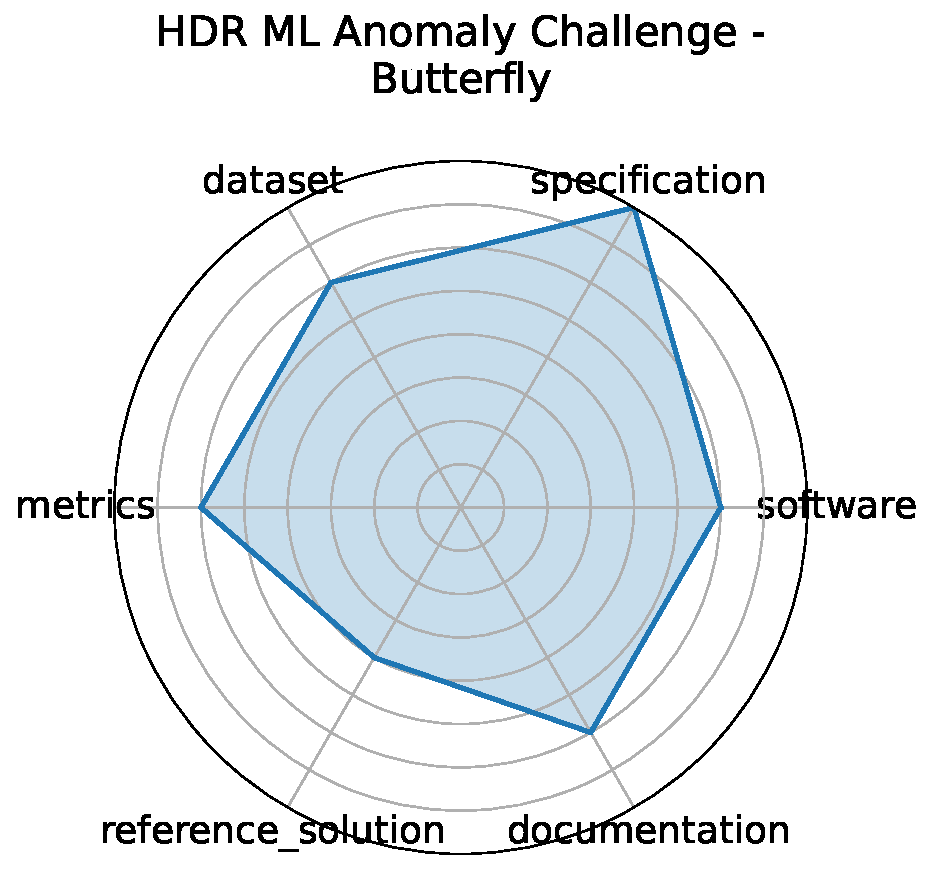
\includegraphics[width=0.2\textwidth]{hdr_ml_anomaly_challenge_-_butterfly_radar.pdf}
}}
\clearpage